\documentclass[1p]{elsarticle_modified}
%\bibliographystyle{elsarticle-num}

%\usepackage[colorlinks]{hyperref}
%\usepackage{abbrmath_seonhwa} %\Abb, \Ascr, \Acal ,\Abf, \Afrak
\usepackage{amsfonts}
\usepackage{amssymb}
\usepackage{amsmath}
\usepackage{amsthm}
\usepackage{scalefnt}
\usepackage{amsbsy}
\usepackage{kotex}
\usepackage{caption}
\usepackage{subfig}
\usepackage{color}
\usepackage{graphicx}
\usepackage{xcolor} %% white, black, red, green, blue, cyan, magenta, yellow
\usepackage{float}
\usepackage{setspace}
\usepackage{hyperref}

\usepackage{tikz}
\usetikzlibrary{arrows}

\usepackage{multirow}
\usepackage{array} % fixed length table
\usepackage{hhline}

%%%%%%%%%%%%%%%%%%%%%
\makeatletter
\renewcommand*\env@matrix[1][\arraystretch]{%
	\edef\arraystretch{#1}%
	\hskip -\arraycolsep
	\let\@ifnextchar\new@ifnextchar
	\array{*\c@MaxMatrixCols c}}
\makeatother %https://tex.stackexchange.com/questions/14071/how-can-i-increase-the-line-spacing-in-a-matrix
%%%%%%%%%%%%%%%

\usepackage[normalem]{ulem}

\newcommand{\msout}[1]{\ifmmode\text{\sout{\ensuremath{#1}}}\else\sout{#1}\fi}
%SOURCE: \msout is \stkout macro in https://tex.stackexchange.com/questions/20609/strikeout-in-math-mode

\newcommand{\cancel}[1]{
	\ifmmode
	{\color{red}\msout{#1}}
	\else
	{\color{red}\sout{#1}}
	\fi
}

\newcommand{\add}[1]{
	{\color{blue}\uwave{#1}}
}

\newcommand{\replace}[2]{
	\ifmmode
	{\color{red}\msout{#1}}{\color{blue}\uwave{#2}}
	\else
	{\color{red}\sout{#1}}{\color{blue}\uwave{#2}}
	\fi
}

\newcommand{\Sol}{\mathcal{S}} %segment
\newcommand{\D}{D} %diagram
\newcommand{\A}{\mathcal{A}} %arc


%%%%%%%%%%%%%%%%%%%%%%%%%%%%%5 test

\def\sl{\operatorname{\textup{SL}}(2,\Cbb)}
\def\psl{\operatorname{\textup{PSL}}(2,\Cbb)}
\def\quan{\mkern 1mu \triangleright \mkern 1mu}

\theoremstyle{definition}
\newtheorem{thm}{Theorem}[section]
\newtheorem{prop}[thm]{Proposition}
\newtheorem{lem}[thm]{Lemma}
\newtheorem{ques}[thm]{Question}
\newtheorem{cor}[thm]{Corollary}
\newtheorem{defn}[thm]{Definition}
\newtheorem{exam}[thm]{Example}
\newtheorem{rmk}[thm]{Remark}
\newtheorem{alg}[thm]{Algorithm}

\newcommand{\I}{\sqrt{-1}}
\begin{document}

%\begin{frontmatter}
%
%\title{Boundary parabolic representations of knots up to 8 crossings}
%
%%% Group authors per affiliation:
%\author{Yunhi Cho} 
%\address{Department of Mathematics, University of Seoul, Seoul, Korea}
%\ead{yhcho@uos.ac.kr}
%
%
%\author{Seonhwa Kim} %\fnref{s_kim}}
%\address{Center for Geometry and Physics, Institute for Basic Science, Pohang, 37673, Korea}
%\ead{ryeona17@ibs.re.kr}
%
%\author{Hyuk Kim}
%\address{Department of Mathematical Sciences, Seoul National University, Seoul 08826, Korea}
%\ead{hyukkim@snu.ac.kr}
%
%\author{Seokbeom Yoon}
%\address{Department of Mathematical Sciences, Seoul National University, Seoul, 08826,  Korea}
%\ead{sbyoon15@snu.ac.kr}
%
%\begin{abstract}
%We find all boundary parabolic representation of knots up to 8 crossings.
%
%\end{abstract}
%\begin{keyword}
%    \MSC[2010] 57M25 
%\end{keyword}
%
%\end{frontmatter}

%\linenumbers
%\tableofcontents
%
\newcommand\colored[1]{\textcolor{white}{\rule[-0.35ex]{0.8em}{1.4ex}}\kern-0.8em\color{red} #1}%
%\newcommand\colored[1]{\textcolor{white}{ #1}\kern-2.17ex	\textcolor{white}{ #1}\kern-1.81ex	\textcolor{white}{ #1}\kern-2.15ex\color{red}#1	}

{\Large $\underline{12a_{0721}~(K12a_{0721})}$}

\setlength{\tabcolsep}{10pt}
\renewcommand{\arraystretch}{1.6}
\vspace{1cm}\begin{tabular}{m{100pt}>{\centering\arraybackslash}m{274pt}}
\multirow{5}{120pt}{
	\centering
	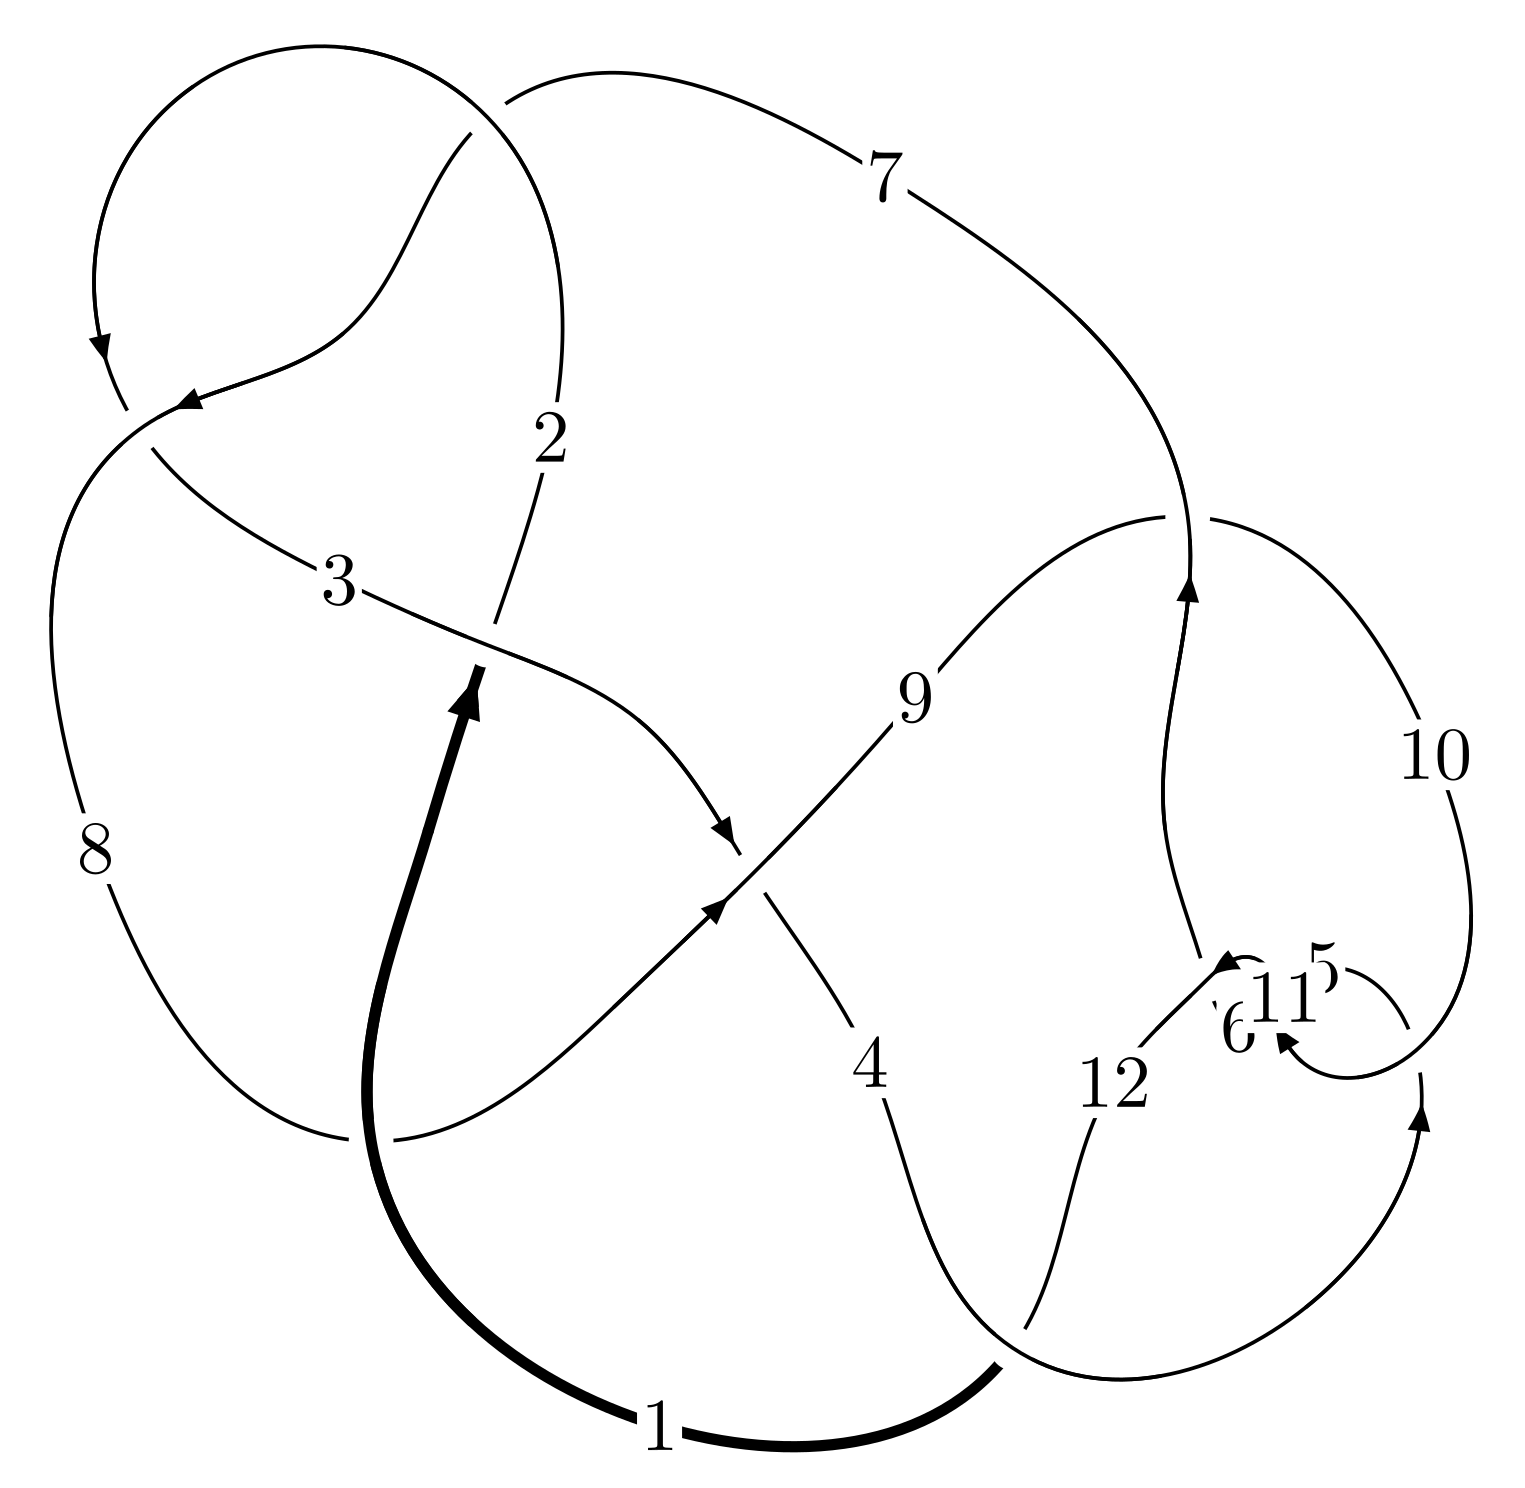
\includegraphics[width=112pt]{../../../GIT/diagram.site/Diagrams/png/1522_12a_0721.png}\\
\ \ \ A knot diagram\footnotemark}&
\allowdisplaybreaks
\textbf{Linearized knot diagam} \\
\cline{2-2}
 &
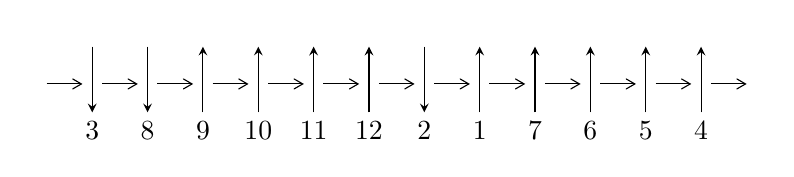
\begin{tikzpicture}[x=20pt, y=17pt]
	% nodes
	\node (C0) at (0, 0) {};
	\node (C1) at (1, 0) {};
	\node (C1U) at (1, +1) {};
	\node (C1D) at (1, -1) {3};

	\node (C2) at (2, 0) {};
	\node (C2U) at (2, +1) {};
	\node (C2D) at (2, -1) {8};

	\node (C3) at (3, 0) {};
	\node (C3U) at (3, +1) {};
	\node (C3D) at (3, -1) {9};

	\node (C4) at (4, 0) {};
	\node (C4U) at (4, +1) {};
	\node (C4D) at (4, -1) {10};

	\node (C5) at (5, 0) {};
	\node (C5U) at (5, +1) {};
	\node (C5D) at (5, -1) {11};

	\node (C6) at (6, 0) {};
	\node (C6U) at (6, +1) {};
	\node (C6D) at (6, -1) {12};

	\node (C7) at (7, 0) {};
	\node (C7U) at (7, +1) {};
	\node (C7D) at (7, -1) {2};

	\node (C8) at (8, 0) {};
	\node (C8U) at (8, +1) {};
	\node (C8D) at (8, -1) {1};

	\node (C9) at (9, 0) {};
	\node (C9U) at (9, +1) {};
	\node (C9D) at (9, -1) {7};

	\node (C10) at (10, 0) {};
	\node (C10U) at (10, +1) {};
	\node (C10D) at (10, -1) {6};

	\node (C11) at (11, 0) {};
	\node (C11U) at (11, +1) {};
	\node (C11D) at (11, -1) {5};

	\node (C12) at (12, 0) {};
	\node (C12U) at (12, +1) {};
	\node (C12D) at (12, -1) {4};
	\node (C13) at (13, 0) {};

	% arrows
	\draw[->,>={angle 60}]
	(C0) edge (C1) (C1) edge (C2) (C2) edge (C3) (C3) edge (C4) (C4) edge (C5) (C5) edge (C6) (C6) edge (C7) (C7) edge (C8) (C8) edge (C9) (C9) edge (C10) (C10) edge (C11) (C11) edge (C12) (C12) edge (C13) ;	\draw[->,>=stealth]
	(C1U) edge (C1D) (C2U) edge (C2D) (C3D) edge (C3U) (C4D) edge (C4U) (C5D) edge (C5U) (C6D) edge (C6U) (C7U) edge (C7D) (C8D) edge (C8U) (C9D) edge (C9U) (C10D) edge (C10U) (C11D) edge (C11U) (C12D) edge (C12U) ;
	\end{tikzpicture} \\
\hhline{~~} \\& 
\textbf{Solving Sequence} \\ \cline{2-2} 
 &
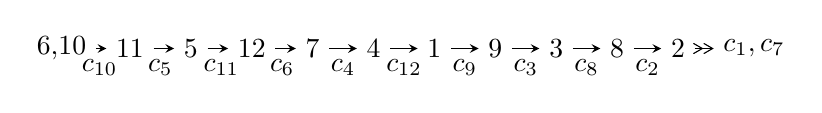
\begin{tikzpicture}[x=22pt, y=7pt]
	% node
	\node (A0) at (-1/8, 0) {6,10};
	\node (A1) at (1, 0) {11};
	\node (A2) at (2, 0) {5};
	\node (A3) at (3, 0) {12};
	\node (A4) at (4, 0) {7};
	\node (A5) at (5, 0) {4};
	\node (A6) at (6, 0) {1};
	\node (A7) at (7, 0) {9};
	\node (A8) at (8, 0) {3};
	\node (A9) at (9, 0) {8};
	\node (A10) at (10, 0) {2};
	\node (C1) at (1/2, -1) {$c_{10}$};
	\node (C2) at (3/2, -1) {$c_{5}$};
	\node (C3) at (5/2, -1) {$c_{11}$};
	\node (C4) at (7/2, -1) {$c_{6}$};
	\node (C5) at (9/2, -1) {$c_{4}$};
	\node (C6) at (11/2, -1) {$c_{12}$};
	\node (C7) at (13/2, -1) {$c_{9}$};
	\node (C8) at (15/2, -1) {$c_{3}$};
	\node (C9) at (17/2, -1) {$c_{8}$};
	\node (C10) at (19/2, -1) {$c_{2}$};
	\node (A11) at (45/4, 0) {$c_{1},c_{7}$};

	% edge
	\draw[->,>=stealth]	
	(A0) edge (A1) (A1) edge (A2) (A2) edge (A3) (A3) edge (A4) (A4) edge (A5) (A5) edge (A6) (A6) edge (A7) (A7) edge (A8) (A8) edge (A9) (A9) edge (A10) ;
	\draw[->>,>={angle 60}]	
	(A10) edge (A11);
\end{tikzpicture} \\ 

\end{tabular} \\

\footnotetext{
The image of knot diagram is generated by the software ``\textbf{Draw programme}" developed by Andrew Bartholomew(\url{http://www.layer8.co.uk/maths/draw/index.htm\#Running-draw}), where we modified some parts for our purpose(\url{https://github.com/CATsTAILs/LinksPainter}).
}\phantom \\ \newline 
\centering \textbf{Ideals for irreducible components\footnotemark of $X_{\text{par}}$} 
 
\begin{align*}
I^u_{1}&=\langle 
u^{85}+u^{84}+\cdots+u+1\rangle \\
\\
\end{align*}
\raggedright * 1 irreducible components of $\dim_{\mathbb{C}}=0$, with total 85 representations.\\
\footnotetext{All coefficients of polynomials are rational numbers. But the coefficients are sometimes approximated in decimal forms when there is not enough margin.}
\newpage
\renewcommand{\arraystretch}{1}
\centering \section*{I. $I^u_{1}= \langle u^{85}+u^{84}+\cdots+u+1 \rangle$}
\flushleft \textbf{(i) Arc colorings}\\
\begin{tabular}{m{7pt} m{180pt} m{7pt} m{180pt} }
\flushright $a_{6}=$&$\begin{pmatrix}0\\u\end{pmatrix}$ \\
\flushright $a_{10}=$&$\begin{pmatrix}1\\0\end{pmatrix}$ \\
\flushright $a_{11}=$&$\begin{pmatrix}1\\- u^2\end{pmatrix}$ \\
\flushright $a_{5}=$&$\begin{pmatrix}- u\\u^3+u\end{pmatrix}$ \\
\flushright $a_{12}=$&$\begin{pmatrix}u^2+1\\- u^4-2 u^2\end{pmatrix}$ \\
\flushright $a_{7}=$&$\begin{pmatrix}u^5+2 u^3+u\\- u^7-3 u^5-2 u^3+u\end{pmatrix}$ \\
\flushright $a_{4}=$&$\begin{pmatrix}- u^3-2 u\\u^3+u\end{pmatrix}$ \\
\flushright $a_{1}=$&$\begin{pmatrix}- u^{10}-5 u^8-8 u^6-3 u^4+3 u^2+1\\u^{10}+4 u^8+5 u^6-3 u^2\end{pmatrix}$ \\
\flushright $a_{9}=$&$\begin{pmatrix}- u^{12}-5 u^{10}-9 u^8-6 u^6+u^2+1\\u^{14}+6 u^{12}+13 u^{10}+10 u^8-2 u^6-4 u^4+u^2\end{pmatrix}$ \\
\flushright $a_{3}=$&$\begin{pmatrix}u^{29}+12 u^{27}+\cdots-6 u^3-3 u\\- u^{31}-13 u^{29}+\cdots+24 u^7+u\end{pmatrix}$ \\
\flushright $a_{8}=$&$\begin{pmatrix}- u^{34}-15 u^{32}+\cdots-3 u^2+1\\u^{34}+14 u^{32}+\cdots+8 u^4+u^2\end{pmatrix}$ \\
\flushright $a_{2}=$&$\begin{pmatrix}u^{70}+29 u^{68}+\cdots+9 u^4+1\\- u^{72}-30 u^{70}+\cdots-6 u^4-2 u^2\end{pmatrix}$\\&\end{tabular}
\flushleft \textbf{(ii) Obstruction class $= -1$}\\~\\
\flushleft \textbf{(iii) Cusp Shapes $= 4 u^{84}+4 u^{83}+\cdots-8 u+6$}\\~\\
\newpage\renewcommand{\arraystretch}{1}
\flushleft \textbf{(iv) u-Polynomials at the component}\newline \\
\begin{tabular}{m{50pt}|m{274pt}}
Crossings & \hspace{64pt}u-Polynomials at each crossing \\
\hline $$\begin{aligned}c_{1}\end{aligned}$$&$\begin{aligned}
&u^{85}+41 u^{84}+\cdots+3 u+1
\end{aligned}$\\
\hline $$\begin{aligned}c_{2},c_{7}\end{aligned}$$&$\begin{aligned}
&u^{85}+u^{84}+\cdots- u-1
\end{aligned}$\\
\hline $$\begin{aligned}c_{3}\end{aligned}$$&$\begin{aligned}
&u^{85}- u^{84}+\cdots-3 u-1
\end{aligned}$\\
\hline $$\begin{aligned}c_{4},c_{6}\end{aligned}$$&$\begin{aligned}
&u^{85}+u^{84}+\cdots-3 u-2
\end{aligned}$\\
\hline $$\begin{aligned}c_{5},c_{10},c_{11}\end{aligned}$$&$\begin{aligned}
&u^{85}- u^{84}+\cdots+u-1
\end{aligned}$\\
\hline $$\begin{aligned}c_{8}\end{aligned}$$&$\begin{aligned}
&u^{85}+3 u^{84}+\cdots-703 u-192
\end{aligned}$\\
\hline $$\begin{aligned}c_{9},c_{12}\end{aligned}$$&$\begin{aligned}
&u^{85}+7 u^{84}+\cdots+433 u+37
\end{aligned}$\\
\hline
\end{tabular}\\~\\
\newpage\renewcommand{\arraystretch}{1}
\flushleft \textbf{(v) Riley Polynomials at the component}\newline \\
\begin{tabular}{m{50pt}|m{274pt}}
Crossings & \hspace{64pt}Riley Polynomials at each crossing \\
\hline $$\begin{aligned}c_{1}\end{aligned}$$&$\begin{aligned}
&y^{85}+7 y^{84}+\cdots-21 y-1
\end{aligned}$\\
\hline $$\begin{aligned}c_{2},c_{7}\end{aligned}$$&$\begin{aligned}
&y^{85}-41 y^{84}+\cdots+3 y-1
\end{aligned}$\\
\hline $$\begin{aligned}c_{3}\end{aligned}$$&$\begin{aligned}
&y^{85}- y^{84}+\cdots+67 y-1
\end{aligned}$\\
\hline $$\begin{aligned}c_{4},c_{6}\end{aligned}$$&$\begin{aligned}
&y^{85}-45 y^{84}+\cdots+9 y-4
\end{aligned}$\\
\hline $$\begin{aligned}c_{5},c_{10},c_{11}\end{aligned}$$&$\begin{aligned}
&y^{85}+71 y^{84}+\cdots+3 y-1
\end{aligned}$\\
\hline $$\begin{aligned}c_{8}\end{aligned}$$&$\begin{aligned}
&y^{85}+27 y^{84}+\cdots+92545 y-36864
\end{aligned}$\\
\hline $$\begin{aligned}c_{9},c_{12}\end{aligned}$$&$\begin{aligned}
&y^{85}+59 y^{84}+\cdots-33697 y-1369
\end{aligned}$\\
\hline
\end{tabular}\\~\\
\newpage\flushleft \textbf{(vi) Complex Volumes and Cusp Shapes}
$$\begin{array}{c|c|c}  
\text{Solutions to }I^u_{1}& \I (\text{vol} + \sqrt{-1}CS) & \text{Cusp shape}\\
 \hline 
\begin{aligned}
u &= -0.248900 + 1.008010 I\end{aligned}
 & -5.94190 + 0.14890 I & \phantom{-0.000000 } 0 \\ \hline\begin{aligned}
u &= -0.248900 - 1.008010 I\end{aligned}
 & -5.94190 - 0.14890 I & \phantom{-0.000000 } 0 \\ \hline\begin{aligned}
u &= -0.297171 + 1.034020 I\end{aligned}
 & -4.01353 + 7.94113 I & \phantom{-0.000000 } 0 \\ \hline\begin{aligned}
u &= -0.297171 - 1.034020 I\end{aligned}
 & -4.01353 - 7.94113 I & \phantom{-0.000000 } 0 \\ \hline\begin{aligned}
u &= \phantom{-}0.280740 + 1.047720 I\end{aligned}
 & -1.61529 - 3.02389 I & \phantom{-0.000000 } 0 \\ \hline\begin{aligned}
u &= \phantom{-}0.280740 - 1.047720 I\end{aligned}
 & -1.61529 + 3.02389 I & \phantom{-0.000000 } 0 \\ \hline\begin{aligned}
u &= \phantom{-}0.270441 + 1.112840 I\end{aligned}
 & -0.089929 - 1.275270 I & \phantom{-0.000000 } 0 \\ \hline\begin{aligned}
u &= \phantom{-}0.270441 - 1.112840 I\end{aligned}
 & -0.089929 + 1.275270 I & \phantom{-0.000000 } 0 \\ \hline\begin{aligned}
u &= -0.278034 + 1.156140 I\end{aligned}
 & -0.94658 - 3.20959 I & \phantom{-0.000000 } 0 \\ \hline\begin{aligned}
u &= -0.278034 - 1.156140 I\end{aligned}
 & -0.94658 + 3.20959 I & \phantom{-0.000000 } 0 \\ \hline\begin{aligned}
u &= \phantom{-}0.209551 + 0.776333 I\end{aligned}
 & -6.17352 + 0.11601 I & -1.51814 - 0.75097 I \\ \hline\begin{aligned}
u &= \phantom{-}0.209551 - 0.776333 I\end{aligned}
 & -6.17352 - 0.11601 I & -1.51814 + 0.75097 I \\ \hline\begin{aligned}
u &= -0.781173 + 0.165218 I\end{aligned}
 & -1.36801 - 11.97790 I & \phantom{-}5.82993 + 9.11891 I \\ \hline\begin{aligned}
u &= -0.781173 - 0.165218 I\end{aligned}
 & -1.36801 + 11.97790 I & \phantom{-}5.82993 - 9.11891 I \\ \hline\begin{aligned}
u &= \phantom{-}0.775804 + 0.160398 I\end{aligned}
 & \phantom{-}1.06779 + 6.99922 I & \phantom{-}9.02457 - 5.56636 I \\ \hline\begin{aligned}
u &= \phantom{-}0.775804 - 0.160398 I\end{aligned}
 & \phantom{-}1.06779 - 6.99922 I & \phantom{-}9.02457 + 5.56636 I \\ \hline\begin{aligned}
u &= -0.766023 + 0.170399 I\end{aligned}
 & -3.38713 - 4.04703 I & \phantom{-}2.85028 + 3.33634 I \\ \hline\begin{aligned}
u &= -0.766023 - 0.170399 I\end{aligned}
 & -3.38713 + 4.04703 I & \phantom{-}2.85028 - 3.33634 I \\ \hline\begin{aligned}
u &= -0.778318 + 0.031728 I\end{aligned}
 & \phantom{-}4.10355 - 5.77938 I & \phantom{-}10.92900 + 6.00912 I \\ \hline\begin{aligned}
u &= -0.778318 - 0.031728 I\end{aligned}
 & \phantom{-}4.10355 + 5.77938 I & \phantom{-}10.92900 - 6.00912 I \\ \hline\begin{aligned}
u &= \phantom{-}0.764543 + 0.137328 I\end{aligned}
 & \phantom{-}2.81551 + 5.13000 I & \phantom{-}10.71873 - 6.57822 I \\ \hline\begin{aligned}
u &= \phantom{-}0.764543 - 0.137328 I\end{aligned}
 & \phantom{-}2.81551 - 5.13000 I & \phantom{-}10.71873 + 6.57822 I \\ \hline\begin{aligned}
u &= \phantom{-}0.772607 + 0.016397 I\end{aligned}
 & \phantom{-}5.85261 + 1.00201 I & \phantom{-}14.4008 - 0.7177 I \\ \hline\begin{aligned}
u &= \phantom{-}0.772607 - 0.016397 I\end{aligned}
 & \phantom{-}5.85261 - 1.00201 I & \phantom{-}14.4008 + 0.7177 I \\ \hline\begin{aligned}
u &= \phantom{-}0.264885 + 0.713873 I\end{aligned}
 & -4.48668 + 7.92179 I & \phantom{-}1.27242 - 7.67068 I \\ \hline\begin{aligned}
u &= \phantom{-}0.264885 - 0.713873 I\end{aligned}
 & -4.48668 - 7.92179 I & \phantom{-}1.27242 + 7.67068 I \\ \hline\begin{aligned}
u &= -0.750929 + 0.115587 I\end{aligned}
 & \phantom{-}2.17145 - 0.56664 I & \phantom{-}9.65396 + 0.21560 I \\ \hline\begin{aligned}
u &= -0.750929 - 0.115587 I\end{aligned}
 & \phantom{-}2.17145 + 0.56664 I & \phantom{-}9.65396 - 0.21560 I \\ \hline\begin{aligned}
u &= \phantom{-}0.719433 + 0.187623 I\end{aligned}
 & -4.06922 + 3.45026 I & \phantom{-}2.04119 - 4.45417 I \\ \hline\begin{aligned}
u &= \phantom{-}0.719433 - 0.187623 I\end{aligned}
 & -4.06922 - 3.45026 I & \phantom{-}2.04119 + 4.45417 I\\
 \hline 
 \end{array}$$\newpage$$\begin{array}{c|c|c}  
\text{Solutions to }I^u_{1}& \I (\text{vol} + \sqrt{-1}CS) & \text{Cusp shape}\\
 \hline 
\begin{aligned}
u &= -0.228274 + 0.698343 I\end{aligned}
 & -2.02866 - 3.11378 I & \phantom{-}4.29634 + 4.05625 I \\ \hline\begin{aligned}
u &= -0.228274 - 0.698343 I\end{aligned}
 & -2.02866 + 3.11378 I & \phantom{-}4.29634 - 4.05625 I \\ \hline\begin{aligned}
u &= -0.326512 + 1.230870 I\end{aligned}
 & \phantom{-}0.41498 + 1.78773 I & \phantom{-0.000000 } 0 \\ \hline\begin{aligned}
u &= -0.326512 - 1.230870 I\end{aligned}
 & \phantom{-}0.41498 - 1.78773 I & \phantom{-0.000000 } 0 \\ \hline\begin{aligned}
u &= -0.184745 + 1.263020 I\end{aligned}
 & -3.07305 - 2.43438 I & \phantom{-0.000000 } 0 \\ \hline\begin{aligned}
u &= -0.184745 - 1.263020 I\end{aligned}
 & -3.07305 + 2.43438 I & \phantom{-0.000000 } 0 \\ \hline\begin{aligned}
u &= \phantom{-}0.688445 + 0.200059 I\end{aligned}
 & -2.66519 - 4.42958 I & \phantom{-}4.16803 + 2.23694 I \\ \hline\begin{aligned}
u &= \phantom{-}0.688445 - 0.200059 I\end{aligned}
 & -2.66519 + 4.42958 I & \phantom{-}4.16803 - 2.23694 I \\ \hline\begin{aligned}
u &= -0.691627 + 0.177718 I\end{aligned}
 & -0.102256 - 0.240928 I & \phantom{-}7.49528 + 1.37110 I \\ \hline\begin{aligned}
u &= -0.691627 - 0.177718 I\end{aligned}
 & -0.102256 + 0.240928 I & \phantom{-}7.49528 - 1.37110 I \\ \hline\begin{aligned}
u &= \phantom{-}0.324883 + 1.246210 I\end{aligned}
 & \phantom{-}2.05753 + 2.96009 I & \phantom{-0.000000 } 0 \\ \hline\begin{aligned}
u &= \phantom{-}0.324883 - 1.246210 I\end{aligned}
 & \phantom{-}2.05753 - 2.96009 I & \phantom{-0.000000 } 0 \\ \hline\begin{aligned}
u &= \phantom{-}0.116828 + 1.284750 I\end{aligned}
 & -6.28256 - 0.70523 I & \phantom{-0.000000 } 0 \\ \hline\begin{aligned}
u &= \phantom{-}0.116828 - 1.284750 I\end{aligned}
 & -6.28256 + 0.70523 I & \phantom{-0.000000 } 0 \\ \hline\begin{aligned}
u &= -0.699942\phantom{ +0.000000I}\end{aligned}
 & \phantom{-}1.55328\phantom{ +0.000000I} & \phantom{-}6.87670\phantom{ +0.000000I} \\ \hline\begin{aligned}
u &= \phantom{-}0.329649 + 1.271860 I\end{aligned}
 & \phantom{-}1.85314 + 4.97870 I & \phantom{-0.000000 } 0 \\ \hline\begin{aligned}
u &= \phantom{-}0.329649 - 1.271860 I\end{aligned}
 & \phantom{-}1.85314 - 4.97870 I & \phantom{-0.000000 } 0 \\ \hline\begin{aligned}
u &= -0.290553 + 1.282560 I\end{aligned}
 & -2.46212 - 3.58115 I & \phantom{-0.000000 } 0 \\ \hline\begin{aligned}
u &= -0.290553 - 1.282560 I\end{aligned}
 & -2.46212 + 3.58115 I & \phantom{-0.000000 } 0 \\ \hline\begin{aligned}
u &= \phantom{-}0.182008 + 1.306080 I\end{aligned}
 & -5.59206 + 6.55252 I & \phantom{-0.000000 } 0 \\ \hline\begin{aligned}
u &= \phantom{-}0.182008 - 1.306080 I\end{aligned}
 & -5.59206 - 6.55252 I & \phantom{-0.000000 } 0 \\ \hline\begin{aligned}
u &= -0.334981 + 1.281900 I\end{aligned}
 & \phantom{-}0.01669 - 9.79487 I & \phantom{-0.000000 } 0 \\ \hline\begin{aligned}
u &= -0.334981 - 1.281900 I\end{aligned}
 & \phantom{-}0.01669 + 9.79487 I & \phantom{-0.000000 } 0 \\ \hline\begin{aligned}
u &= -0.317650 + 1.339370 I\end{aligned}
 & -2.41072 - 4.43457 I & \phantom{-0.000000 } 0 \\ \hline\begin{aligned}
u &= -0.317650 - 1.339370 I\end{aligned}
 & -2.41072 + 4.43457 I & \phantom{-0.000000 } 0 \\ \hline\begin{aligned}
u &= -0.013172 + 1.384380 I\end{aligned}
 & -6.34751 - 2.22482 I & \phantom{-0.000000 } 0 \\ \hline\begin{aligned}
u &= -0.013172 - 1.384380 I\end{aligned}
 & -6.34751 + 2.22482 I & \phantom{-0.000000 } 0 \\ \hline\begin{aligned}
u &= \phantom{-}0.324897 + 1.349170 I\end{aligned}
 & -1.86872 + 9.07355 I & \phantom{-0.000000 } 0 \\ \hline\begin{aligned}
u &= \phantom{-}0.324897 - 1.349170 I\end{aligned}
 & -1.86872 - 9.07355 I & \phantom{-0.000000 } 0 \\ \hline\begin{aligned}
u &= -0.293142 + 1.358620 I\end{aligned}
 & -4.94324 - 3.84382 I & \phantom{-0.000000 } 0\\
 \hline 
 \end{array}$$\newpage$$\begin{array}{c|c|c}  
\text{Solutions to }I^u_{1}& \I (\text{vol} + \sqrt{-1}CS) & \text{Cusp shape}\\
 \hline 
\begin{aligned}
u &= -0.293142 - 1.358620 I\end{aligned}
 & -4.94324 + 3.84382 I & \phantom{-0.000000 } 0 \\ \hline\begin{aligned}
u &= \phantom{-}0.288385 + 1.364890 I\end{aligned}
 & -7.59509 - 0.86185 I & \phantom{-0.000000 } 0 \\ \hline\begin{aligned}
u &= \phantom{-}0.288385 - 1.364890 I\end{aligned}
 & -7.59509 + 0.86185 I & \phantom{-0.000000 } 0 \\ \hline\begin{aligned}
u &= \phantom{-}0.301046 + 1.365670 I\end{aligned}
 & -8.97185 + 7.16378 I & \phantom{-0.000000 } 0 \\ \hline\begin{aligned}
u &= \phantom{-}0.301046 - 1.365670 I\end{aligned}
 & -8.97185 - 7.16378 I & \phantom{-0.000000 } 0 \\ \hline\begin{aligned}
u &= \phantom{-}0.328741 + 1.361380 I\end{aligned}
 & -3.73450 + 10.99570 I & \phantom{-0.000000 } 0 \\ \hline\begin{aligned}
u &= \phantom{-}0.328741 - 1.361380 I\end{aligned}
 & -3.73450 - 10.99570 I & \phantom{-0.000000 } 0 \\ \hline\begin{aligned}
u &= -0.323051 + 1.364830 I\end{aligned}
 & -8.23465 - 7.99145 I & \phantom{-0.000000 } 0 \\ \hline\begin{aligned}
u &= -0.323051 - 1.364830 I\end{aligned}
 & -8.23465 + 7.99145 I & \phantom{-0.000000 } 0 \\ \hline\begin{aligned}
u &= -0.330797 + 1.364300 I\end{aligned}
 & -6.1963 - 15.9996 I & \phantom{-0.000000 } 0 \\ \hline\begin{aligned}
u &= -0.330797 - 1.364300 I\end{aligned}
 & -6.1963 + 15.9996 I & \phantom{-0.000000 } 0 \\ \hline\begin{aligned}
u &= -0.023413 + 1.410440 I\end{aligned}
 & -8.46842 - 3.63559 I & \phantom{-0.000000 } 0 \\ \hline\begin{aligned}
u &= -0.023413 - 1.410440 I\end{aligned}
 & -8.46842 + 3.63559 I & \phantom{-0.000000 } 0 \\ \hline\begin{aligned}
u &= \phantom{-}0.02698 + 1.41604 I\end{aligned}
 & -11.02750 + 8.52728 I & \phantom{-0.000000 } 0 \\ \hline\begin{aligned}
u &= \phantom{-}0.02698 - 1.41604 I\end{aligned}
 & -11.02750 - 8.52728 I & \phantom{-0.000000 } 0 \\ \hline\begin{aligned}
u &= \phantom{-}0.01432 + 1.41634 I\end{aligned}
 & -12.76900 + 0.46813 I & \phantom{-0.000000 } 0 \\ \hline\begin{aligned}
u &= \phantom{-}0.01432 - 1.41634 I\end{aligned}
 & -12.76900 - 0.46813 I & \phantom{-0.000000 } 0 \\ \hline\begin{aligned}
u &= -0.159545 + 0.546638 I\end{aligned}
 & -0.43421 - 1.85967 I & \phantom{-}4.91547 + 5.62191 I \\ \hline\begin{aligned}
u &= -0.159545 - 0.546638 I\end{aligned}
 & -0.43421 + 1.85967 I & \phantom{-}4.91547 - 5.62191 I \\ \hline\begin{aligned}
u &= \phantom{-}0.408138 + 0.257025 I\end{aligned}
 & -0.93232 + 4.40586 I & \phantom{-}5.40236 - 8.36399 I \\ \hline\begin{aligned}
u &= \phantom{-}0.408138 - 0.257025 I\end{aligned}
 & -0.93232 - 4.40586 I & \phantom{-}5.40236 + 8.36399 I \\ \hline\begin{aligned}
u &= \phantom{-}0.266823 + 0.380763 I\end{aligned}
 & -1.43413 - 1.94308 I & \phantom{-}2.89552 - 0.96140 I \\ \hline\begin{aligned}
u &= \phantom{-}0.266823 - 0.380763 I\end{aligned}
 & -1.43413 + 1.94308 I & \phantom{-}2.89552 + 0.96140 I \\ \hline\begin{aligned}
u &= -0.391169 + 0.128683 I\end{aligned}
 & \phantom{-}0.923187 - 0.319535 I & \phantom{-}11.07004 + 2.67367 I \\ \hline\begin{aligned}
u &= -0.391169 - 0.128683 I\end{aligned}
 & \phantom{-}0.923187 + 0.319535 I & \phantom{-}11.07004 - 2.67367 I\\
 \hline 
 \end{array}$$\newpage
\newpage\renewcommand{\arraystretch}{1}
\centering \section*{ II. u-Polynomials}
\begin{tabular}{m{50pt}|m{274pt}}
Crossings & \hspace{64pt}u-Polynomials at each crossing \\
\hline $$\begin{aligned}c_{1}\end{aligned}$$&$\begin{aligned}
&u^{85}+41 u^{84}+\cdots+3 u+1
\end{aligned}$\\
\hline $$\begin{aligned}c_{2},c_{7}\end{aligned}$$&$\begin{aligned}
&u^{85}+u^{84}+\cdots- u-1
\end{aligned}$\\
\hline $$\begin{aligned}c_{3}\end{aligned}$$&$\begin{aligned}
&u^{85}- u^{84}+\cdots-3 u-1
\end{aligned}$\\
\hline $$\begin{aligned}c_{4},c_{6}\end{aligned}$$&$\begin{aligned}
&u^{85}+u^{84}+\cdots-3 u-2
\end{aligned}$\\
\hline $$\begin{aligned}c_{5},c_{10},c_{11}\end{aligned}$$&$\begin{aligned}
&u^{85}- u^{84}+\cdots+u-1
\end{aligned}$\\
\hline $$\begin{aligned}c_{8}\end{aligned}$$&$\begin{aligned}
&u^{85}+3 u^{84}+\cdots-703 u-192
\end{aligned}$\\
\hline $$\begin{aligned}c_{9},c_{12}\end{aligned}$$&$\begin{aligned}
&u^{85}+7 u^{84}+\cdots+433 u+37
\end{aligned}$\\
\hline
\end{tabular}\newpage\renewcommand{\arraystretch}{1}
\centering \section*{ III. Riley Polynomials}
\begin{tabular}{m{50pt}|m{274pt}}
Crossings & \hspace{64pt}Riley Polynomials at each crossing \\
\hline $$\begin{aligned}c_{1}\end{aligned}$$&$\begin{aligned}
&y^{85}+7 y^{84}+\cdots-21 y-1
\end{aligned}$\\
\hline $$\begin{aligned}c_{2},c_{7}\end{aligned}$$&$\begin{aligned}
&y^{85}-41 y^{84}+\cdots+3 y-1
\end{aligned}$\\
\hline $$\begin{aligned}c_{3}\end{aligned}$$&$\begin{aligned}
&y^{85}- y^{84}+\cdots+67 y-1
\end{aligned}$\\
\hline $$\begin{aligned}c_{4},c_{6}\end{aligned}$$&$\begin{aligned}
&y^{85}-45 y^{84}+\cdots+9 y-4
\end{aligned}$\\
\hline $$\begin{aligned}c_{5},c_{10},c_{11}\end{aligned}$$&$\begin{aligned}
&y^{85}+71 y^{84}+\cdots+3 y-1
\end{aligned}$\\
\hline $$\begin{aligned}c_{8}\end{aligned}$$&$\begin{aligned}
&y^{85}+27 y^{84}+\cdots+92545 y-36864
\end{aligned}$\\
\hline $$\begin{aligned}c_{9},c_{12}\end{aligned}$$&$\begin{aligned}
&y^{85}+59 y^{84}+\cdots-33697 y-1369
\end{aligned}$\\
\hline
\end{tabular}
\vskip 2pc
\end{document}